% This document is part of the transientdict project.
% Copyright 2013 the authors.

\documentclass[12pt]{emulateapj}
\usepackage{xspace}
\usepackage{graphicx}
%\usepackage{epsfig}
\usepackage{times}
\usepackage{natbib}
\usepackage{amsfonts}
\usepackage{amsmath}
\usepackage{amsbsy}
\usepackage{bm}
\usepackage{hyperref}
\usepackage{url}
%\usepackage{subfigure}
\usepackage{microtype}
\usepackage{rotating}
\usepackage{booktabs}
\usepackage{threeparttable}
\usepackage{tabularx}
\usepackage{subfigure}


%\usepackage{longtable}%\usepackage[stable]{footmisc}
%\usepackage{color}
%\bibliographystyle{apj}

% MB: I added xspace so that we don't have to use '\ ' after the commands
% For commands that may or may not stay inside a math environment, we can 
% also use \ensuremath
\newcommand{\project}[1]{\textsl{#1}\xspace}
\newcommand{\fermi}{\project{Fermi}\xspace}
\newcommand{\rxte}{\project{RXTE}\xspace}
\newcommand{\given}{\ensuremath{\,|\,}}
\newcommand{\dd}{\ensuremath{\mathrm{d}}}
\newcommand{\counts}{\ensuremath{y}}
\newcommand{\pars}{\ensuremath{\theta}}
\newcommand{\mean}{\ensuremath{\lambda}}
\newcommand{\likelihood}{\ensuremath{{\mathcal L}}}
\newcommand{\Poisson}{\ensuremath{{\mathcal P}}}
\newcommand{\Uniform}{\ensuremath{{\mathcal U}}}
\newcommand{\bg}{\ensuremath{\mathrm{bg}}}
\newcommand{\word}{\ensuremath{\phi}}
\newcommand{\zsq}{\ensuremath{Z^2_n}}
\newcommand{\stingray}{\texttt{stingray}\xspace}
\newcommand{\maltpynt}{\texttt{whatever-name-ex-maltpynt-gets}\xspace}
\newcommand{\python}{\texttt{Python}\xspace}
\newcommand{\astropy}{\texttt{astropy}\xspace}
\newcommand{\lightcurve}{\texttt{Lightcurve}\xspace}

%\newcommand{\bs}{\boldsymbol}

\begin{document}

\title{\stingray: A modern \python\ Library For Spectral Timing}

\author{D. Huppenkothen\altaffilmark{1, 2, 3}, M. Bachetti\altaffilmark{4}, A. Stevens\altaffilmark{}, OTHER CO-AUTHORS!}
 
\altaffiltext{1}{Center for Cosmology and Particle Physics, Department of Physics, New York University, 4 Washington Place, New York, NY 10003, USA \\
}
  \altaffiltext{2}{Center for Data Science, New York University, 65 5h Avenue, 7th Floor, New York, NY 10003}
  \altaffiltext{3}{E-mail: daniela.huppenkothen@nyu.edu}
\altaffiltext{4}{INAF-Osservatorio Astronomico di Cagliari, via della Scienza 5, I-09047 Selargius (CA), Italy}
\altaffiltext{5}{}
\altaffiltext{}{}
\altaffiltext{}{}


\begin{abstract}
% This abstract could be more exciting, I think.
This paper describes the design, implementation and usage of \stingray, a library in \python built to perform time series analysis and related tasks on astronomical light curves. 
Its core functionality comprises a large range of Fourier analysis techniques commonly used in Spectral Timing, as well as extensions for analysing pulsar data, simulating data sets, and statistical modelling. 
Its modular build allows for easy extensions and we aim for the library to be a platform for future development. 
Here, we describe its Python classes and functions in detail, as well as give practical example using astronomical data sets. 
The code is well-tested, with a test coverage of currently 95\%.

\end{abstract}

\keywords{methods:statistics}

\section{Introduction}

Variability is one of the key diagnostics in understanding the underlying physics of the dynamics and emission processes from astronomical objects. 
The detection of periodic variations in the radio flux of certain objects has led to the ground-breaking discovery of pulsars. Similarly, accurately describing of dips in stellar light curves has led to the discovery of thousands of exoplanets. 
In high-energy astrophysics, particularly the study of black holes and neutron stars, the scientific developments of recent years have brought a growing understanding that time and wavelength are intricately linked. 
Different spectral components react differently to changes in accretion rate and dynamics, leading to time lags, correlated variability and higher-order effects. 
This has led to the study of accretion disks, in particular those of Active Galactic Nuclei (AGN), via reverberation mapping. 
Understanding how the emission at various wavelengths changes with time is crucial for testing and expanding our understanding of General Relativity in the strong gravity limit, the dense matter equation of state and other fundamental questions in astrophysics.

Despite decades of research, the field is fragmented in terms of software; there is no commonly accepted, up-to-date framework for the core data analysis tasks involved in (spectral) timing. Code is generally siloed within groups, leading to a general lack of reproducibility of scientific results. 
The NASA library \texttt{xronos} is, to our knowledge, the only significant open-source library in this field, and has several shortcomings. 
In particular, it performs only a few of the most basic tasks, and it has not been maintained since 2004. 
Here, we introduce \stingray, a lightweight library built entirely in \python and based on \astropy functionality, to address the lack of well-tested, well-documented software for spectral timing. 
\stingray aims to make many of the core Fourier analysis tools used in timing analysis available to a large range of researchers while providing a common platform for new methods and tools as they enter the field. 
It includes the most relevant functionality in its core package, while extending that functionality in its subpackages in several ways, allowing for easy modeling of light curves and power spectra, simulation of synthetic data sets and pulsar timing. 
The modularity of its classes allows for easy incorporation of existing \stingray functionality into larger data analysis workflows and pipelines, while being easily extensible for cases that the library currently does not cover. 
As of v1.0, it includes basic functionality depends exclusively on \texttt{numpy} [REF], \texttt{scipy}[REF] and \texttt{astropy}[REF], with optional plotting functionality supplied by \texttt{matplotlib}[REF], \texttt{seaborn}[REF]  and \texttt{corner}, and optional sampling methods by \texttt{emcee}[REF].

This paper describes \stingray v1.0, released on [ADD DATE]. 
As with most open-source packages, \stingray is under continuous development and welcomes contributions from the community.
The paper layout is as follows: 
In Section \ref{sec:general_package}, we describe the general package structure. 
In Section \ref{sec:core}, we detail the package's core functionality in Fourier analysis and introduce basic classes for storing light curves and Fourier spectra of various types. 
In Section \ref{sec:modeling}, we extend this core functionality with \stingray's modeling framework and in Section \ref{sec:simulator}, we show how users can easily simulate data sets from models. 
Sections \ref{sec:pulsar} lays out the functionality for analysing pulsar data, and Section{ref:dave} details existing connections to a graphical user interface currently being developed in parallel to \stingray. 
Finally, in Sections \ref{sec:development} and \ref{sec:future} we lay out the development process, testing and documentation environments as well as our future development plans. 
In each section, we present examples of the functionality described based on real-world data sets.


\section{General Package Framework}
\label{sec:general_package}





\section{Core Functionality}
\label{sec:core}

\stingray imports its core functions and classes from the top level package. 
These classes define the basic data structures such as light curves and cross- as well as power spectra that are used in much of the higher-level functionality provided in the sub-packages. 
Additionally, it incorporates a large range of utilities for dealing with Good Time Intervals (GTIs) as well as input and output of data sets.


\begin{table}[hbtp]
%\renewcommand{\arraystretch}{1.0}
\footnotesize
\caption{Parameters for the simulated data set}
\begin{threeparttable} 
\begin{tabularx}{8.5cm}{p{2.5cm}p{4.0cm}p{2.0cm}}
\toprule
\bf{Parameter} & \bf{Description} &\bf{Value} \\ \midrule
$A_{\mathrm{PL}}$ & Power law amplitude & $0.1$ \\
$\alpha$ & Power law spectral index & 1.0 \\
$A_{\mathrm{QPO}}$ & QPO amplitude &  $1.0$ \\
$\nu_0$ & QPO centroid frequency & $2.0 \,\mathrm{Hz}$ \\
$\gamma$ & QPO full width at half-maximum &$1 \,\mathrm{Hz}$ \\
 \bottomrule
\end{tabularx}
   \begin{tablenotes}
      \item{}
\end{tablenotes}
\end{threeparttable}
\label{table:parameters}
\end{table}

\subsection{The \texttt{Lightcurve} class}
\label{sec:lightcurve}

\begin{figure*}
\begin{center}
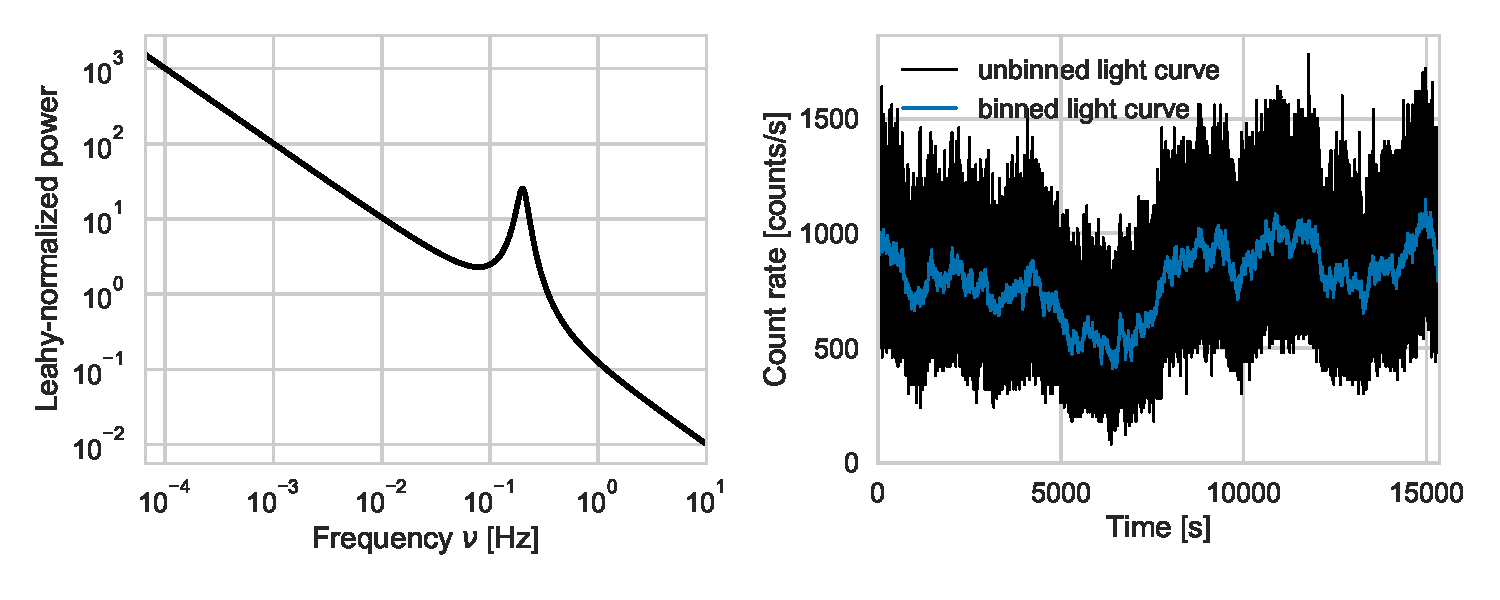
\includegraphics[width=\textwidth]{../figures/lc.png}
\caption{Power spectrum model (left) used for generation of a simulated light curve (right) using the method from \citet{timmer1995}. The underlying power spectrum consists of a power law and a Lorentzian. We use the Poisson distribution with the flux in each bin to approximate the observed photon counting statistics prevalent in X-ray astronomy. In the right panel, we also showcase the binning capabilities of the \texttt{Lightcurve} class.}
\label{fig:scores}
\end{center}
\end{figure*}


We expect \stingray to be used largely on data sets of two forms: (1) event data (i.e. recordings of arrival times of individual photons) or (2) binned light curves. 
The majority of methods in \stingray use binned light curves, which we thus currently consider the default format. The \lightcurve class defines a basic data structure to store binned light curves. Its features include arrays describing time bins and associated (flux or counts) measurements, the number of data points in the light curve, the time resolution and the total duration of the light curve. For unevenly sampled light curves, the time resolution \texttt{dt} will be defined as the median difference between time bin midpoints. Users can pass uncertainties for measurements directly, or pass a string defining the statistical distribution of the data points for automatic calculation. By default, a Poisson distribution is assumed, appropriate for binned event data. 

There are two ways to generate a \texttt{Lightcurve} object: in the standard case, the instrument has recorded a binned time series of $N$ pairs of time stamps and count (rate) or flux values, $\{t_k, c_k \}_{k=1}^{N}$. In this case, one can simply instantiate a \texttt{Lightcurve} object with the keywords \texttt{time} and \texttt{counts} (and optionally \texttt{use\_counts} when the input is in units of counts per second). In cases where the native data format is events (e.g.\ photon arrival times) it is possible to use the static method \texttt{Lightcurve.make\_lightcurve}, passing the array of events as well as a time resolution \texttt{dt} to create a new light curve from the events.

Various operations are implemented for class \lightcurve. In particular, custom behaviour of the $+$ and $-$ operators allows straightforward addition and subtraction of light curves from one another. Assuming the light curves have the same time bins, the $+$ and $-$ operators will add or subtract the flux or counts measurements, respectively, and return a new \lightcurve\ object with the results. Other common operations implemented includes time-shifting the light curve by a constant factor, joining two light curves into a single object, truncating a light curve at a certain time bin, and input/output operations to read or write objects from/to disk in various formats (HDF5, FITS and ASCII are currently supported). For light curves that do not have consecutive time bins, there is a sorting operations, as well as the option to sort the light curve by the ascending or descending flux or counts. 

In addition, we provide support for Good Time Intervals (GTIs) in many methods and implement rebinning the light curve to a new time resolution exceeding the native resolution of the data. In Figure \ref{fig:lightcurve} (right panel), we show an example light curve produced by the texttt{simulator} subpackage (see Section \ref{sec:simulator}) for implementation details). To showcase much of the functionality in the following chapters, we assume a process producing a power spectrum with an intrinsic spectrum comprising a power law and a quasi-periodic oscillation, approximated by a Lorentzian function (Figure \ref{fig:lightcurve}, left panel):

\[
P(\nu) = A_{\mathrm{PL}} \nu^{\alpha} + \frac{A \gamma^2}{\gamma^2 + (\nu - \nu_0)^2} \, .
\]

We use the algorithm from \citet{timmer1995} to generate a light curve with a time resolution of $\delta t = 0.05\,\mathrm{s}$ and a length of $15.36 \,\mathrm{ks}$, amounting to $307200$ data points. The power law has a spectral index of $\alpha = 1.0$, the QPO a centroid frequency of $2 \,\mathrm{Hz}$. The generated light curve has a mean count rate of $400\,\mathrm{counts/s}$ and a fractional rms amplitude of $\mathrm{rms}_\mathrm{frac} = 0.3$. Because the resulting light curve will follow Gaussian uncertainties, we simulate photon counting statistics by drawing from a Poisson distribution for every bin with a rate parameter equal to the simulated flux in that bin. 

The remaining parameters can be found in Table \ref{tab:simdata}\footnote{The full code to reproduce all figures in this paper can be found at \url{https://github.com/stingraysoftware/stingraypaper}}. 


\subsection{The \texttt{Events} class}

\subsection{Cross Spectra and Power Spectra}
\label{sec:csps}

Both the power spectrum and the cross spectrum are standard measures of variability in the wider astronomical community, but have been used in X-ray astronomy in particular to probe a varied set of physical problems, including the properties of the accretion flow onto black holes and neutron stars [REFS]. Both are based on the Fourier transform, where the (complex) Fourier amplitude $a_j$ at frequency $\nu_j$ is defined as

\begin{equation}
a_j = \sum_{k=0}^{N-1}{c_k e^{2\pi i k/N}} \;\;\; j = -\frac{N}{2}, \mathrm{...}, \frac{N}{2} - 1 \; .
\end{equation}

\noindent for a data set of $N$ data points $\{c_k\}_{k=1}^N$. For a single light curve, the \textit{power spectrum}\footnote{A note on language: in signal processing, there is an important distinction to be made between the term \textit{periodogram} and \textit{power spectrum}. More generally, the term \textit{power spectrum} describes the underlying (physical) process that produced an observation. The power spectrum will have a certain shape or form, in astronomy often modelled with Lorentzian or power law-type functions. The \textit{periodogram}, on the other hand, generally denotes a \textit{realization} of the power spectrum, i.e.\ an observed time series derived from an underlying (red noise, QPO, ...) process. Therefore, the squaredFourier transform of an observed light curve is, strictly speaking, a periodogram. However, the term \textit{power spectrum} has a long history within astronomy (and especially in X-ray astronomy) as denoting the squared Fourier amplitudes of an observed light curve. In order to minimize confusion, we continue with this convention, but warn the reader that it is prone to confusion in the larger context of the signal processing literature, as well in circumstances where one must describe both the underlying process and an observed realization of that process.} is defined as the squared absolute value of the Fourier amplitudes of that light curve alone, so that the imaginary parts of the complex Fourier amplitude cancel out (see \citealt{vanderklis1989} for an excellent introduction into Fourier analysis for X-ray astronomy and \citealt{uttley2014} for a more recent review on spectral timing methods in X-ray astronomy):

\begin{equation}
P(\nu_j) = |a_j|^2 \, .
\end{equation}

\noindent The cross spectrum of two light curves $\{c_k\}_{k=1}^N$ and  $\{d_k\}_{k=1}^N$ in terms of its Fourier amplitudes $\{a_j\}_{j=1}^{N/2}$ and  $\{b_j\}_{j=1}^{N/2}$, respectively, is defined as

\begin{equation}
C_{ab,j} = a_j*b_j \, .
\end{equation}

\noindent Notice that because $a_j$ and $b_j$ originate from different light curves, the imaginary part will in general not cancel out for the cross spectrum. However, it should be obvious that the power spectrum is a special case of the cross spectrum, where $\{c_k\}_{k=1}^N = \{d_k\}_{k=1}^N$ and thus  $\{a_j\}_{j=1}^{N/2} = \{b_j\}_{j=1}^{N/2}$. Cross spectra and power spectra are therefore implemented jointly, including a more general class \texttt{Crossspectrum}, and a subclass \texttt{Powerspectrum} that inherits most of the functionality of its super class while minimizing code duplication.

The implementation in texttt{stingray} for both cross- and power spectra makes use of the Discrete Fourier transform as implemented in \texttt{scipy.fftpack}. The resulting Fourier amplitudes are multiplied and normalized according to one of four commonly used normalizations, set using the keyword \texttt{norm}. For a value of \texttt{none}, the unnormalized squared Fourier amplitudes will be returned. Other possible normalizations include Leahy \citep{leahy1984}, fractional rms normalization [REF????] and absolute rms normalization [REF????]. If no GTIs are given within the \texttt{Lightcurve} object, GTIs may be specified in the call to \texttt{Crossspectrum} or \texttt{Powerspectrum}, though for power spectra created from a single light curve, only contiguous GTIs are currently supported, since the Fourier transform requires evenly sampled data to derive statistically sound conclusions. Because in practice, astronomical light curves include the presence of uncorrelated signal between the two light curves $\{c_k\}_{k=1}^N$ and  $\{d_k\}_{k=1}^N$ (e.g.\ in the form of measurement uncertainties), cross spectra should generally be averaged over adjacent Fourier frequency bins or multiple light curve segments, and \stingray\ does currently not allow the calculation of cross spectra on single light curves. Because averaging of multiple light curve segments is common for both power- and cross spectra, the classes \texttt{AveragedCrossspectrum} and \texttt{AveragedPowerspectrum} allow for straightforward calculation of averaged Fourier representation. Both take either a single light curve as well as a  value for the \texttt{segment\_size} keyword, encoding the size of each light curve segment to be averaged, or a list of \texttt{Lightcurve} objects. In addition, both single-light curve spectra as well as the averaged versions support re-binning in frequency space to a new frequency resolution that is coarser than that initially calculated. 


\subsection{Higher-Order Fourier Products}
\label{sec:fourier_others}

\section{The \texttt{modeling} Subpackage}
\label{sec:modeling}

\section{The \texttt{simulator} Subpackage}
\label{sec:simulator}

\section{The \texttt{pulse} Subpackage}
\label{sec:pulsar}
\stingray contains the basic operations to perform the search and characterization of pulsed signals.
(...)
\subsection{Folding}
Among the basic algorithms used in pulsar astronomy, one cannot overstate the importance of Epoch Folding (EF).
The algorithm consists of cutting the signal at every pulse period and summing all sub-intervals in phase. 
An alternative way of seeing it, more useful for photon data, is just a \textit {histogram of pulse phases}.

If the period is exactly correct and assuming a stable pulsation, the signal-to-noise ratio will get better approximately with the square root of the number of summed sub-intervals [REF].
This is the method used to obtain practically all pulse profiles shown in the literature, as most pulsar signals are orders of magnitude below noise level.

The `pulse.pulsar` submodule contains the functionality to calculate the phase given a simple pulse ephemeris consisting of any number of pulse frequency derivatives%
\footnote{For more complicated cases, like binary pulsars or long-term pulsar noise not well described by pulse derivatives, we recommend to look at more focused libraries like \href{https://github.com/nanograv/PINT}{PINT} [REF]}.
Moreover, we have a mechanism to calculate the exposure of single bins in the pulse profile. 
This is particularly useful for very long-period pulsars where the pulsed period is comparable to the length of the GTIs.
The different exposure of pulse bins caused by the absence of signals during GTIs is taken into account in the calculation of the final pulse profile by the folding algorithm, if the user asks for it. 

\subsection{Epoch Folding and \zsq search}
\label{sec:efzsq}
During a search for pulsations, the first step is usually the PDS. 
However, often pulsations do not leave a clear signature above noise level in the PDS, because they are weak or they fall close to bin edges, where the sensitivity is reduced [REF].
Even when they do, the frequency resolution of the PDS is often inadequate to measure precisely the pulse frequency.
Therefore, an additional statistical analysis is needed. 
In this Section, we will describe the Epoch Folding search (EFS).
This search method consists of executing the folding at many trial frequencies around the candidate frequency.
Once the folding is performed, the following statistics is calculated on the profile:
\begin{equation}
\mathcal{S} = \sum_i\frac{(P_i - \overline{P})^2}{\sigma^2}
\end{equation}
where $P_i$ are the bins of the profile, $\overline{P}$ is the mean level of the profile, and $\sigma$ is the standard deviation.
This is the \textit{chi squared} of the actual pulsed profile with respect to a \textit{flat} model.

If there is no pulsation, the chi squared will assume a random value distributed around the number of degrees of freedom $n - 1$ (where $n$ is the number of bins in the profile) with a well defined statistical distribution ($\chi^2_{n - 1}$) that allows an easy calculation of detection limits. 
When a peak is \textit{very unlikely} (meaning that the probability to be obtained by noise is below a certain $\epsilon$), this peak is considered a pulse candidate.
If the frequency resolution is sufficiently high, close to the correct frequency, as described by [Leahy et al. 1983, 1987], the peak in the epoch folding periodogram has the shape of a \textbf{sinc squared function} whose width is driven by the length of the observation.

The epoch folding statistics, however, can give the same value for a pulse profile at the correct frequency and, for example, an harmonic that produces a deviation from a Poisson distribution.
A more effective method is the $Z^2_n$ statistics (Buccheri et al. 1983), which is conceptually similar to EF but has high values when the signal is well described by a small number of \textbf{sinusoidal harmonics}: 

\begin{equation}
\zsq = \dfrac{2}{N} \sum_{k=1}^n \left[{\left(\sum_{j=1}^N \cos k \phi_j\right)}^2 + {\left(\sum_{j=1}^N \sin k \phi_j\right)}^2\right]
\end{equation}

Where $N$ is the number of photons, $n$ is the number of harmonics, $\phi_j$ are the phases corresponding to the event arrival times $t_j$ ($\phi_j = \nu t_j$, where $\nu$ is the pulse frequency).

The \zsq statistics defined in this way, far from the pulsed profile, follows a $\chi^2_n$ distribution, where $n$ is the number of harmonics this time.
This allows, again, to easily calculate thresholds based on the probability of obtaining a given \zsq by pure noise.

The standard \zsq search calculates the phase of each photon and calculates the sinusoidal functions above for each photon.
This is very computationally expensive if the number of photons is high. 
Therefore, in Stingray, the search is performed by binning the pulse profile first and using the phases of the folded profile in the formula above, multiplying the squared sinusoids of the phases of the pulse profile by a weight corresponding to the number of photons at each phase.

\begin{equation}
\zsq \approx \dfrac{2}{\sum_j{w_j}} \sum_{k=1}^n \left[{\left(\sum_{j=1}^m w_j \cos k \phi_j\right)}^2 + {\left(\sum_{j=1}^m w_j \sin k \phi_j\right)}^2\right]
\end{equation}

Since the sinusoids are only executed on a small number of bins, while the epoch folding procedure just consists of a very fast histogram-like operation, the speedup of this new formula is obvious. 
Care must be put into the choice of the number of bins, in order to maintain a good approximation even when the number of harmonics is high. 
We recommend in the documentation to use a number of bins at least 10 times larger than the number of harmonics.

\subsection{Characterization of pulsar behavior}
\label{sec:ephem}
As seen in Section~\ref{sec:efzsq}, the \zsq or the EF periodograms of a perfectly stable pulsation have the shape of a sinc squared function.
\stingray has additional functionality to fit these periodograms with sinc squared or Gaussian models, and find the mean frequency with high precision.

A significant deviation from the expected shape from these peaks in the periodogram can happen if the pulsation is not stable.
Calculating the periodogram is an option to investigate how the pulse phase varies in time.
The periodogram is basically a 2-D histogram of the phase and arrival times of the pulses. 
If the pulsation is stable and the pulse frequency was determined with precision, the periodogram shows vertical stripes corresponding to perfectly aligned pulses.
If the frequency is not as precise, the stripes become more and more diagonal.
If the pulse has a detectable frequency derivative, these stripes bend with a parabolic shape.

A very precise way to determine the exact pulse ephemeris is out of the scope of \stingray. 
However, \stingray has a mechanism to calculate the pulse arrival times (or times of arrival, TOAs) using a pulse template, using the \texttt{fftfit} algorithm used for radio pulsars. 
This is implemented in the \texttt{get\_TOA} function in `stingray.pulse.pulsar`.
Then, the user can use the TOAs with more focused software like Tempo, Tempo2 or PINT.

[Fig. XXXX: a variation of the pulse phase corresponding to a period derivative. ]

\section{Connections to \texttt{DAVE}}
\label{sec:dave}

\section{\maltpynt: command-line interface}
\label{sec:maltpynt}


\section{Development and Integration Environment}
\label{sec:development}

\section{Future Development Plans}
\label{sec:future}

\paragraph{acknowledgements}
DH acknowledges funding from the James Arthur Fellowship at NYU and the Moore-Sloan Data Science Environment at NYU. 
We thank the Lorentz Centre for organizing the workshop that started this collaboration.
\clearpage

\bibliography{stingraypaper}
\bibliographystyle{apj}

\end{document}


